\chapter{IMPLEMENTATION}

\renewcommand{\headrulewidth}{0.5pt}
\renewcommand{\footrulewidth}{0.5pt}
\thispagestyle{plain}
\pagestyle{fancy}
\fancyhf{}
\fancyhead[L]{\textbf{CHAPTER 5}}
\fancyhead[R]{\textbf{Intelligent Traffic System}}
\raggedright
\fancyfoot[L]{From: ITM Vision}
\fancyfoot[R]{Page \thepage}

In the process of real-time multiple-object tracking, it can improve the tracking effect under occlusion by extracting the apparent features of the target and matching the nearest neighbor. At the same time, it also reduces the problem of target ID switches. \\ 
\vspace{3mm}
The MOT models the state of each object and describes the motion of objects in video frames, and the result of tracking allows us to stack trajectories of moving objects across several consecutive frames. \\ 
\vspace{3mm}
In order to solve the vehicle tracking problem, it is necessary to retrain the feature extractor used in the \textbf{DeepSORT Algorithm}, so that it can extract vehicle features well and facilitate the construction of the subsequent correlation matrix. \\ 
\vspace{3mm}
Feature extractor used in the DeepSORT algorithm needs to be retrained on the vehicle reidentification VeRi dataset, so that the improved DeepSORT algorithm is more suitable for the vehicle multitarget tracking task. \\ 
\vspace{3mm}
To overcome shortage of computation power of edge devices, Chen et al suggests using interval multiframe tracking to enhance processing speed, different from the original tracking algorithm that uses the adjacent frames to update the vehicle tracking results, 
we use interval frames to perform updating of the tracking results. \\ 
\vspace{3mm}
To become the part of life of every citizen, the NN-based smart solutions must pass the test of energy-efficiency, small form-factor and affordability. The urgency of achieving these objectives is also evident from the introduction of recent competitions 
such as “low-power image recognition challenge” (LPIRC) which emphasize a balance between accuracy, throughput and power budget. \\ 
\vspace{3mm}
Among these, NVIDIA’s Jetson is very promising and one of the most widely used accelerators for the inference phase of machine learning. Jetson features CPU-GPU heterogeneous architecture where CPU can boot the OS and the CUDA-capable GPU can be quickly 
programmed to accelerate complex machine-learning tasks. Further, it has small form factor, low weight and power consumption which makes it a perfect fit for weight/power-constrained scenarios. \\ 
\vspace{3mm}
Nayak et al suggests that Deep SORT in combination with one stage detectors like YOLO or SSD should be used to implement GPU-based embedded devices such as Jetson TX2, AGX, etc, ... in traffic surveillance systems. \\ 
\vspace{3mm}
Therefore we deploy our system on Jetson platform using TensorRT to optimize the algorithm and leverage CUDA as well as CuDNN.
\begin{figure}[H]
    \centering
    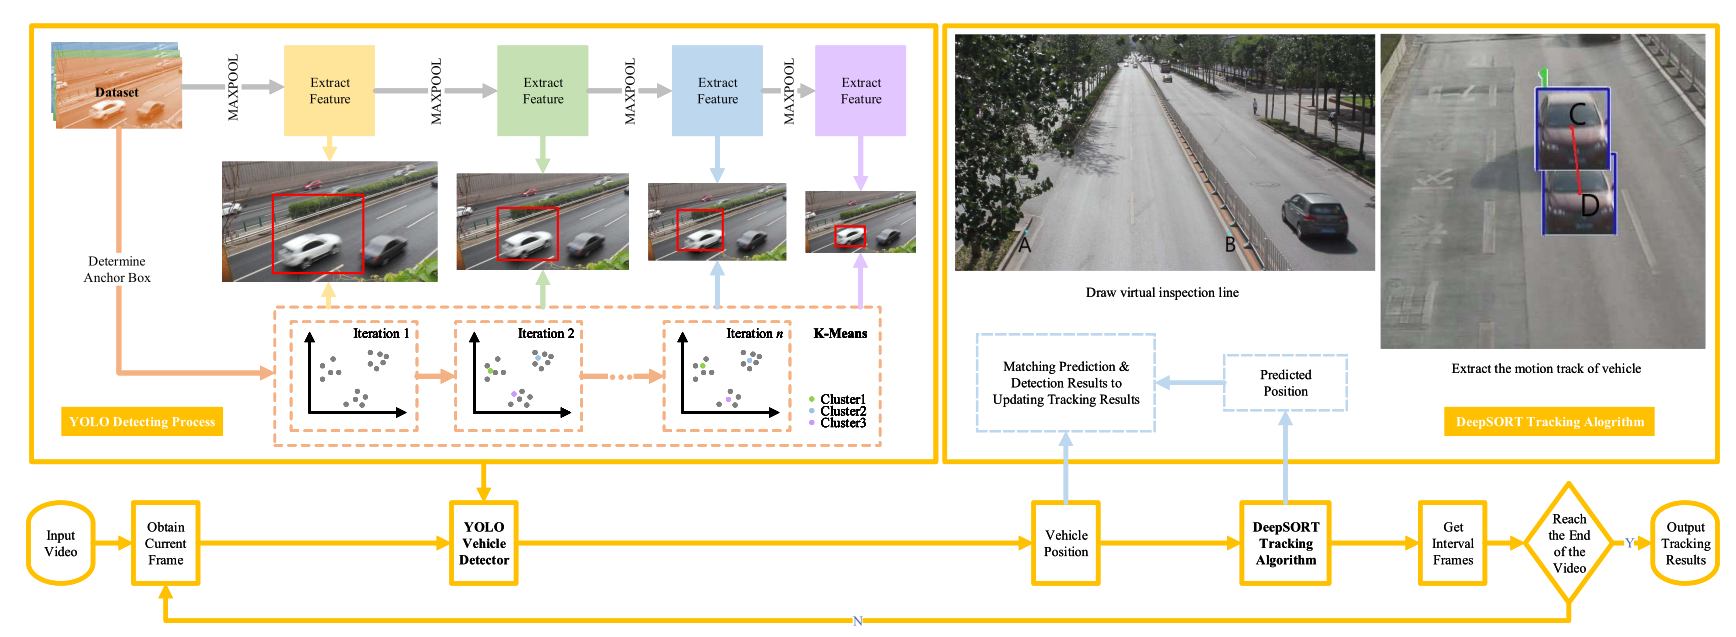
\includegraphics[width=0.6\linewidth]{img/suggest-baseline.png}
    \caption{Suggested Baseline}
\end{figure}
After vehicle is tracked, mapping from pixel space to real world space is occured and then vehicle speed is estimated.
\begin{figure}[H]
    \centering
    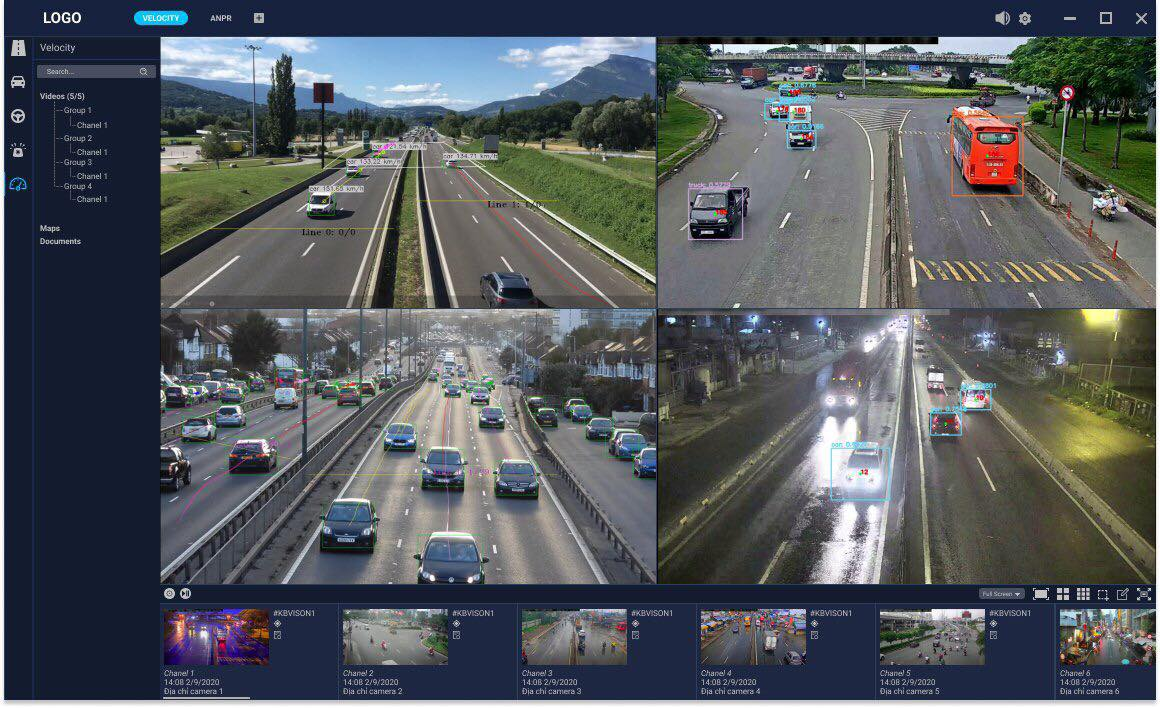
\includegraphics[width=0.6\linewidth]{img/GUI.jpg}
    \caption{GUI Of The System}
\end{figure}
The system makes inferences on Vietnam Traffic Data
\begin{figure}[H]
    \centering
    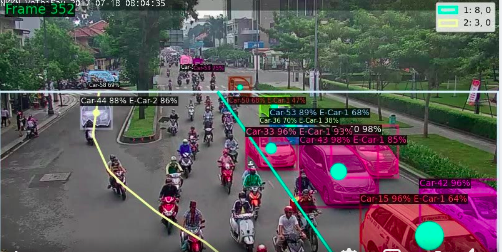
\includegraphics[width=0.6\linewidth]{img/vietnam.png}
    \caption{Vietnam Traffic Data}
\end{figure}